\documentclass[10pt,a4paper]{article}
\usepackage[utf8]{inputenc}
\usepackage{amsmath}
\usepackage{amsthm}
\usepackage{amsfonts}
\usepackage{amssymb}
\usepackage{geometry}
\usepackage{graphicx}
\usepackage{enumitem}
\usepackage{minted}
\usepackage{xcolor}
\definecolor{mygray}{gray}{0.9}
\author{Nicolò Fornari}
\title{Network security}
\newtheorem{remark}{Remark}
\setlength\parindent{0pt}
\def\labelitemi{$\cdot$}

% cool urls
% requires package hyperref
%
% \url{http://...}

% place code in here
% require package minted
%
% \begin{minted}[
% bgcolor=mygray,
% ]{python}
%
% \end{minted}

% include image
% requires package graphicx
%
%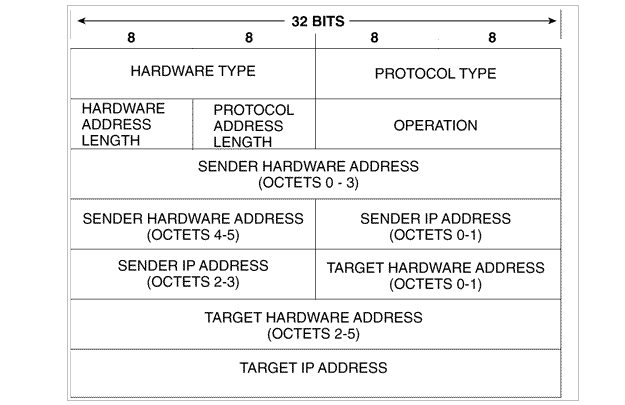
\includegraphics[scale=0.6]{arp.png}


% Handle space in itemize
% requires package enumitem
%
%\begin{itemize}[noitemsep,nolistsep]
%\item aaa
% \item bbb
% \end{itemize}

\begin{document}

\section{Key exchange}

\begin{itemize}
\item TLS\_RSA
\item TLS\_DH\_anon (anonymous)
\item TLS\_PSK (pre shared key)
\item TLS\_SRP (secure remote password)
\end{itemize}

Only these methods provide {\bf forward secrecy} since the public key changes for every instance of the protocol. The last 'e' stands for \textit{ephemeral}.
\begin{itemize}
\item TLS\_DHE
\item TLS\_ECDHE
\end{itemize}
\vspace{1em}
The following methods provide no authentication of server and user, hence suffers from MITM attacks, rarely used
\begin{itemize}
\item TLS\_DH
\item TLS\_ECDH
\end{itemize}
\begin{remark}
These methods can be combined together for instance we can have DHE\_RSA, ECDHE\_PSK, PSK\_RSA etc.
\end{remark}


\subsection{Secure Remote Password}
TLS\_SRP provides {\bf mutual authentication } while TLS with server certificates only authenticates the server to the client.\\
Moreover the user does not need to check the URL being certified since if the server does not know the password the connection can not be established. This prevent phising. \\
Note that using password based authentication does not require reliance of certification authorities.

\section{Block cipher modes}
A block cipher by itself is only suitable for the secure cryptographic transformation (encryption or decryption) of one fixed-length group of bits called a block. A mode of operation describes how to repeatedly apply a cipher's single-block operation to securely transform amounts of data larger than a block.\\\\
Most modes require a unique binary sequence, often called an initialization vector (IV), for each encryption operation. The IV has to be non-repeating and, for some modes, random as well. The initialization vector is used to ensure distinct ciphertexts are produced even when the same plaintext is encrypted multiple times independently with the same key.
\subsection{Electronic Codebook (ECB)}
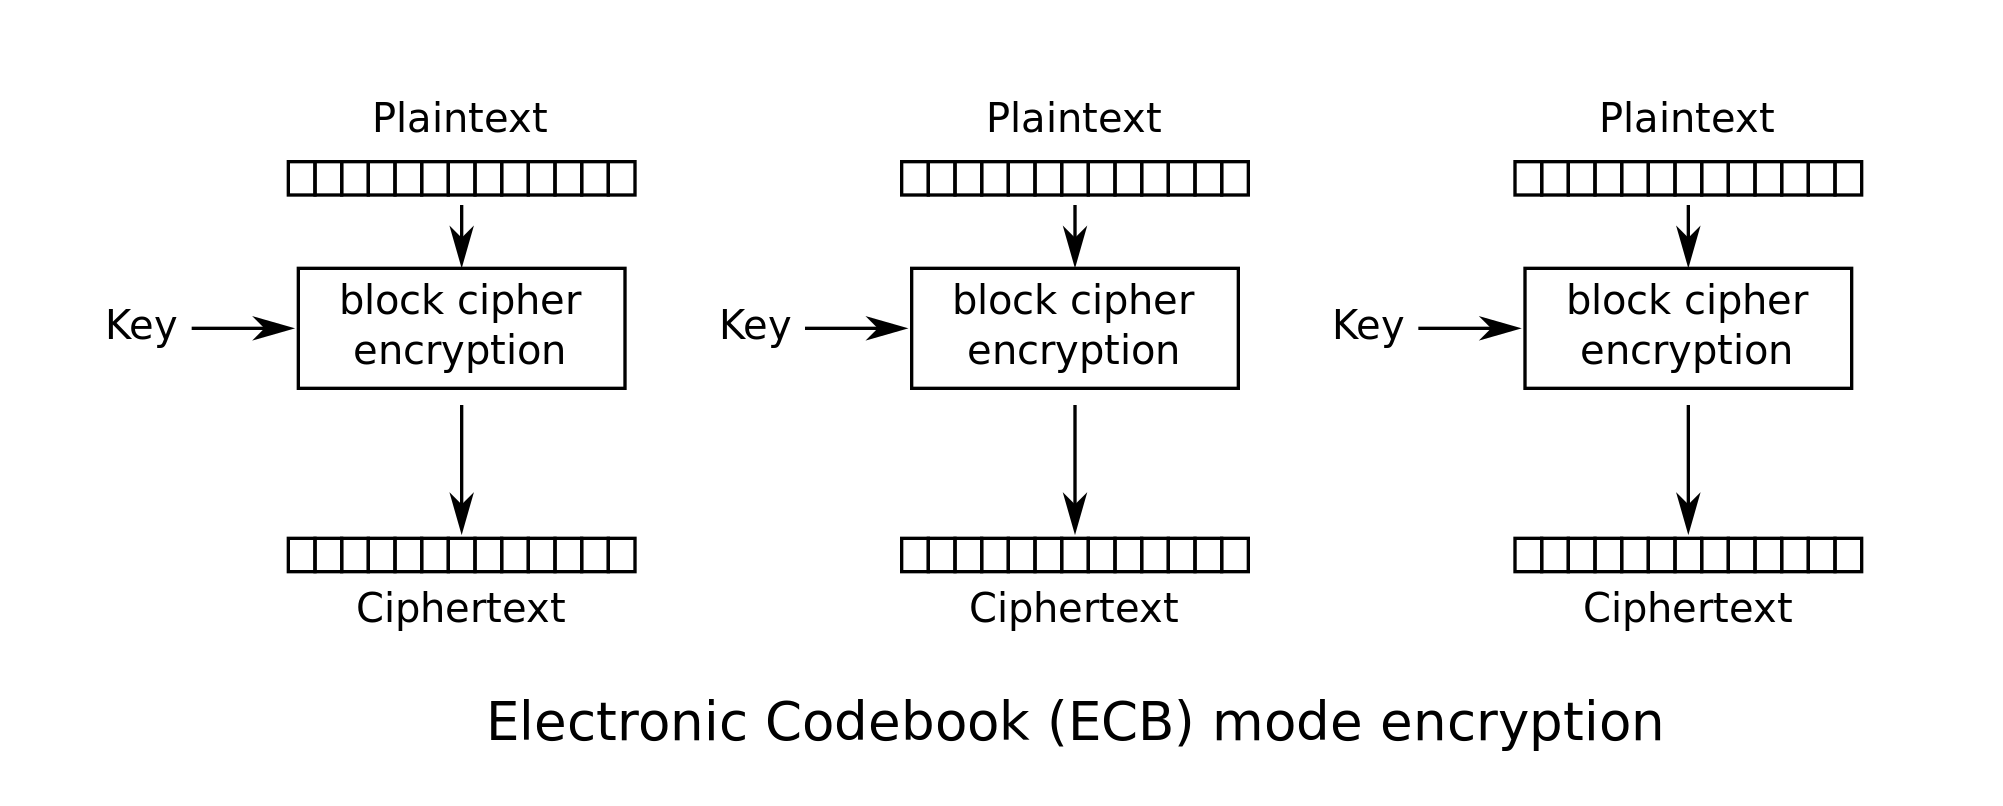
\includegraphics[scale=0.2]{img/ECB.png}
\newline
The message is divided into blocks, and each block is encrypted separately. The disadvantage of this method is that identical plaintext blocks are encrypted into identical ciphertext blocks; thus, it does not hide data patterns well. In some senses, it doesn't provide serious message confidentiality, and it is not recommended for use in cryptographic protocols at all\\\\
Example 1: you see patterns in an image\\
Example 2: headers are standard hence the attacker has pairs (PT,CT) for free!
\begin{remark} it is good to store short information such as password \end{remark}
\subsection{Cipher Block Chaining (CBC)}
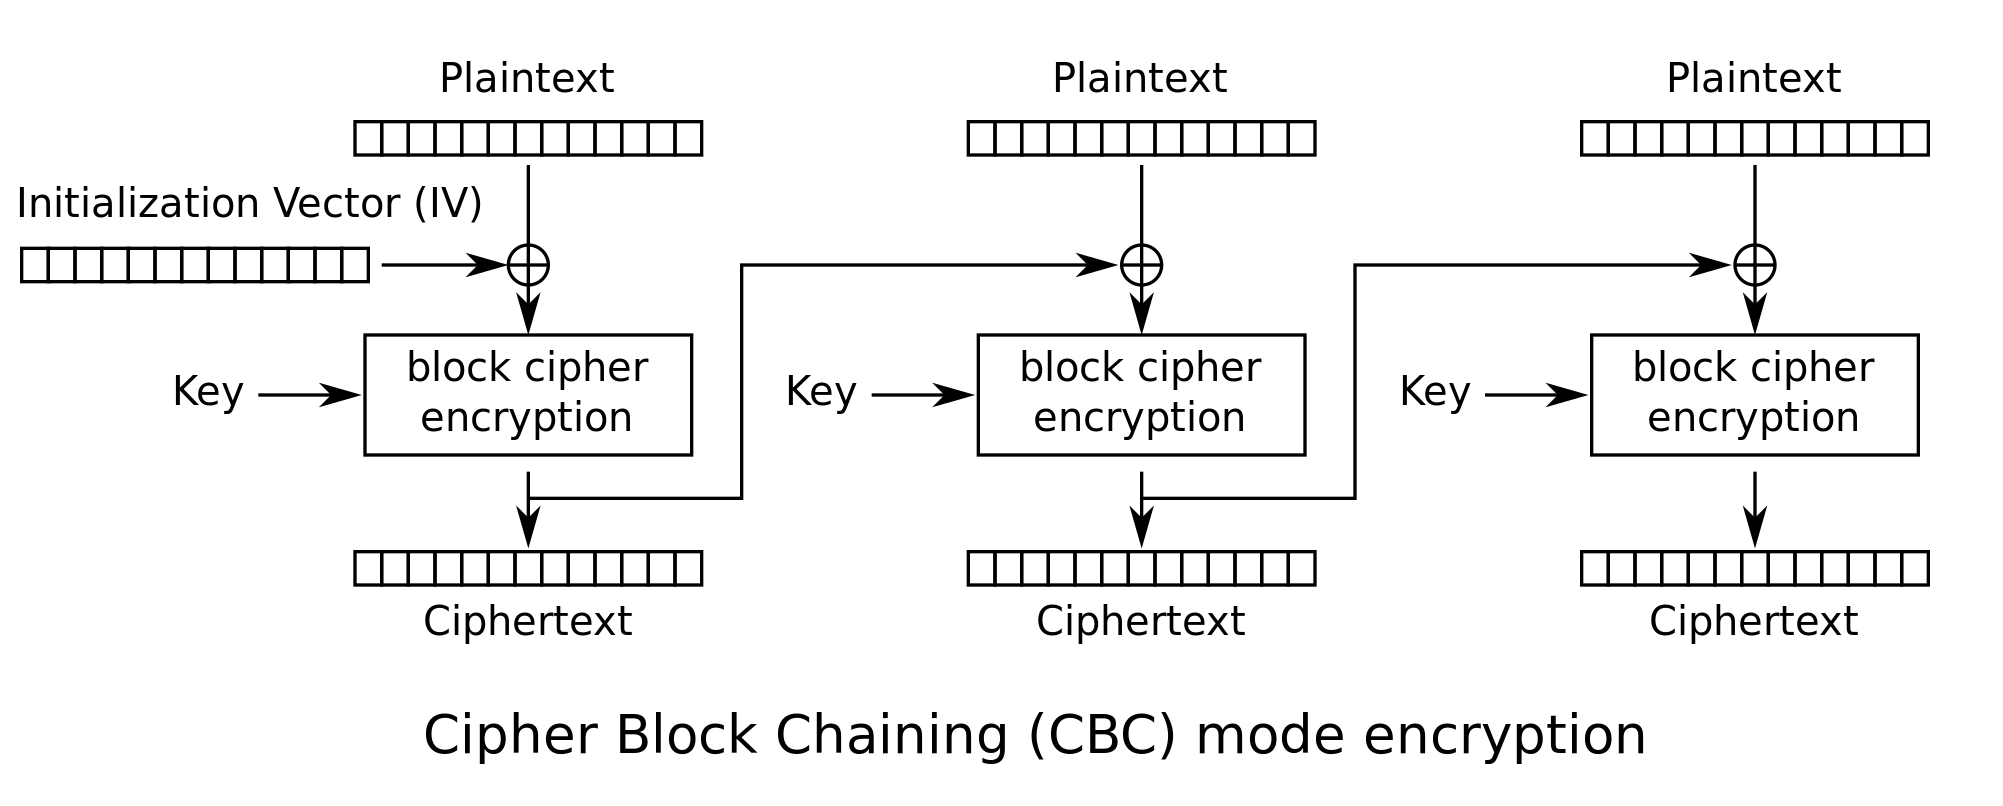
\includegraphics[scale=0.2]{img/CBC.png}
\newline
 In CBC mode, each block of plaintext is XORed with the previous ciphertext block before being encrypted. This way, each ciphertext block depends on all plaintext blocks processed up to that point. To make each message unique, an initialization vector must be used in the first block.
\begin{remark} usually the IV is encrypted with ECB. \end{remark}
\subsection{Propagating Cipher Block Chaining (PCBC)}
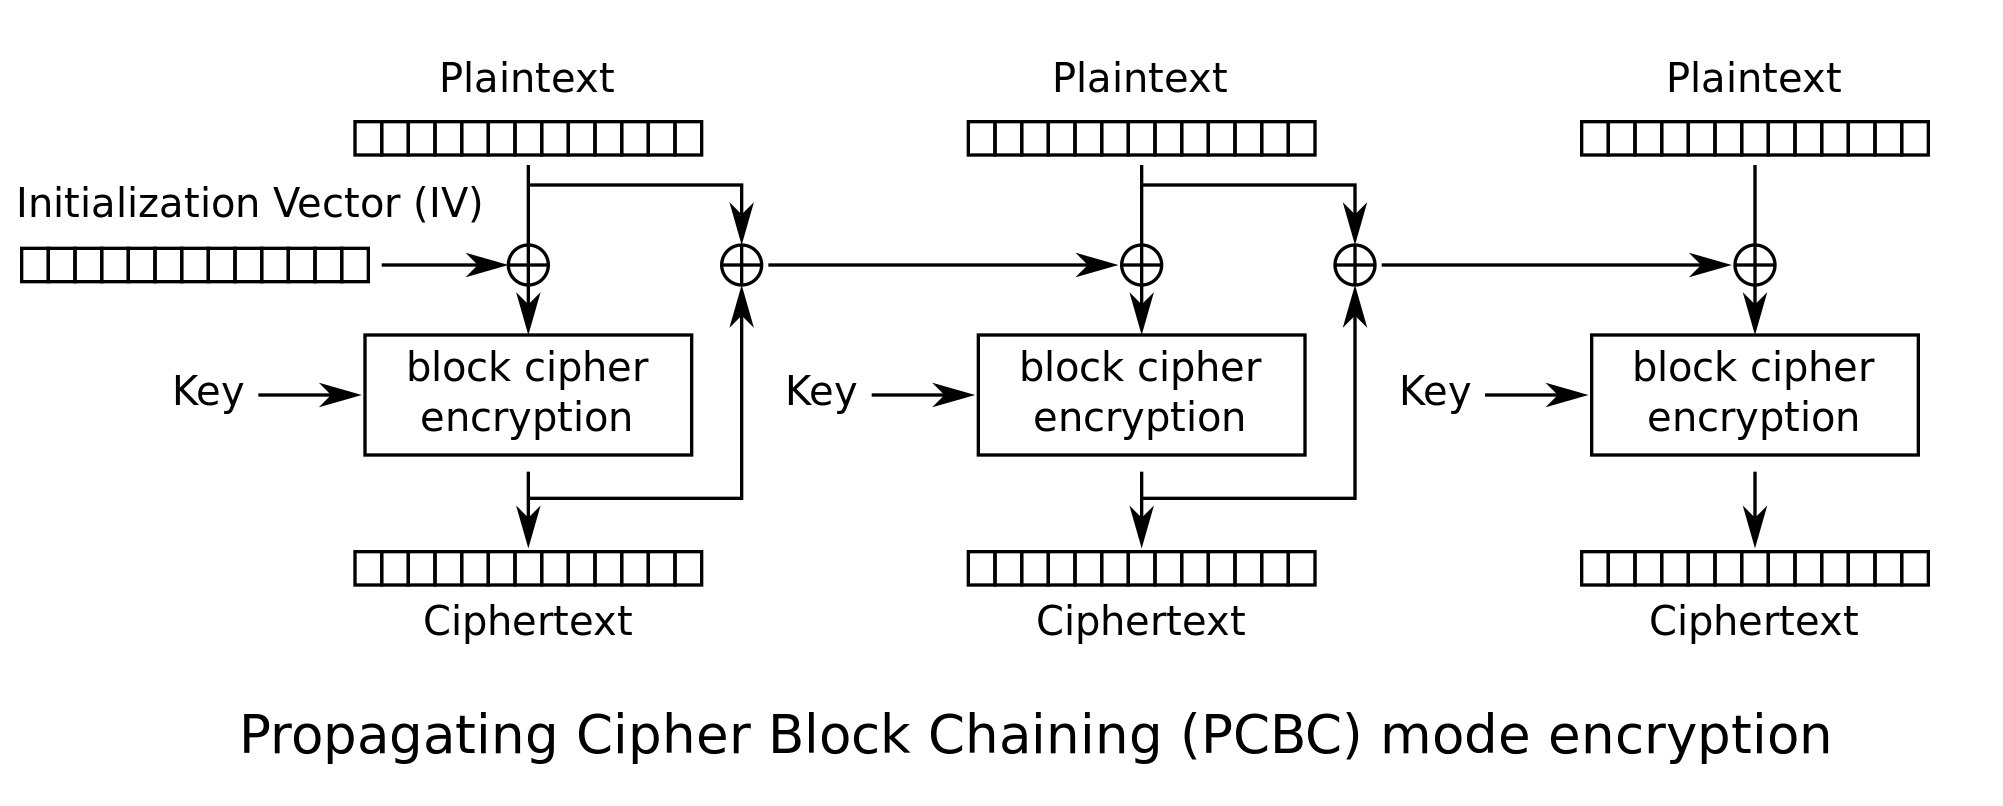
\includegraphics[scale=0.2]{img/PCBC.png}
\newline 
In PCBC mode, each block of plaintext is XORed with both the previous plaintext block and the previous ciphertext block before being encrypted. As with CBC mode, an initialization vector is used in the first block.
\subsection{Cipher Feedback (CFB)}
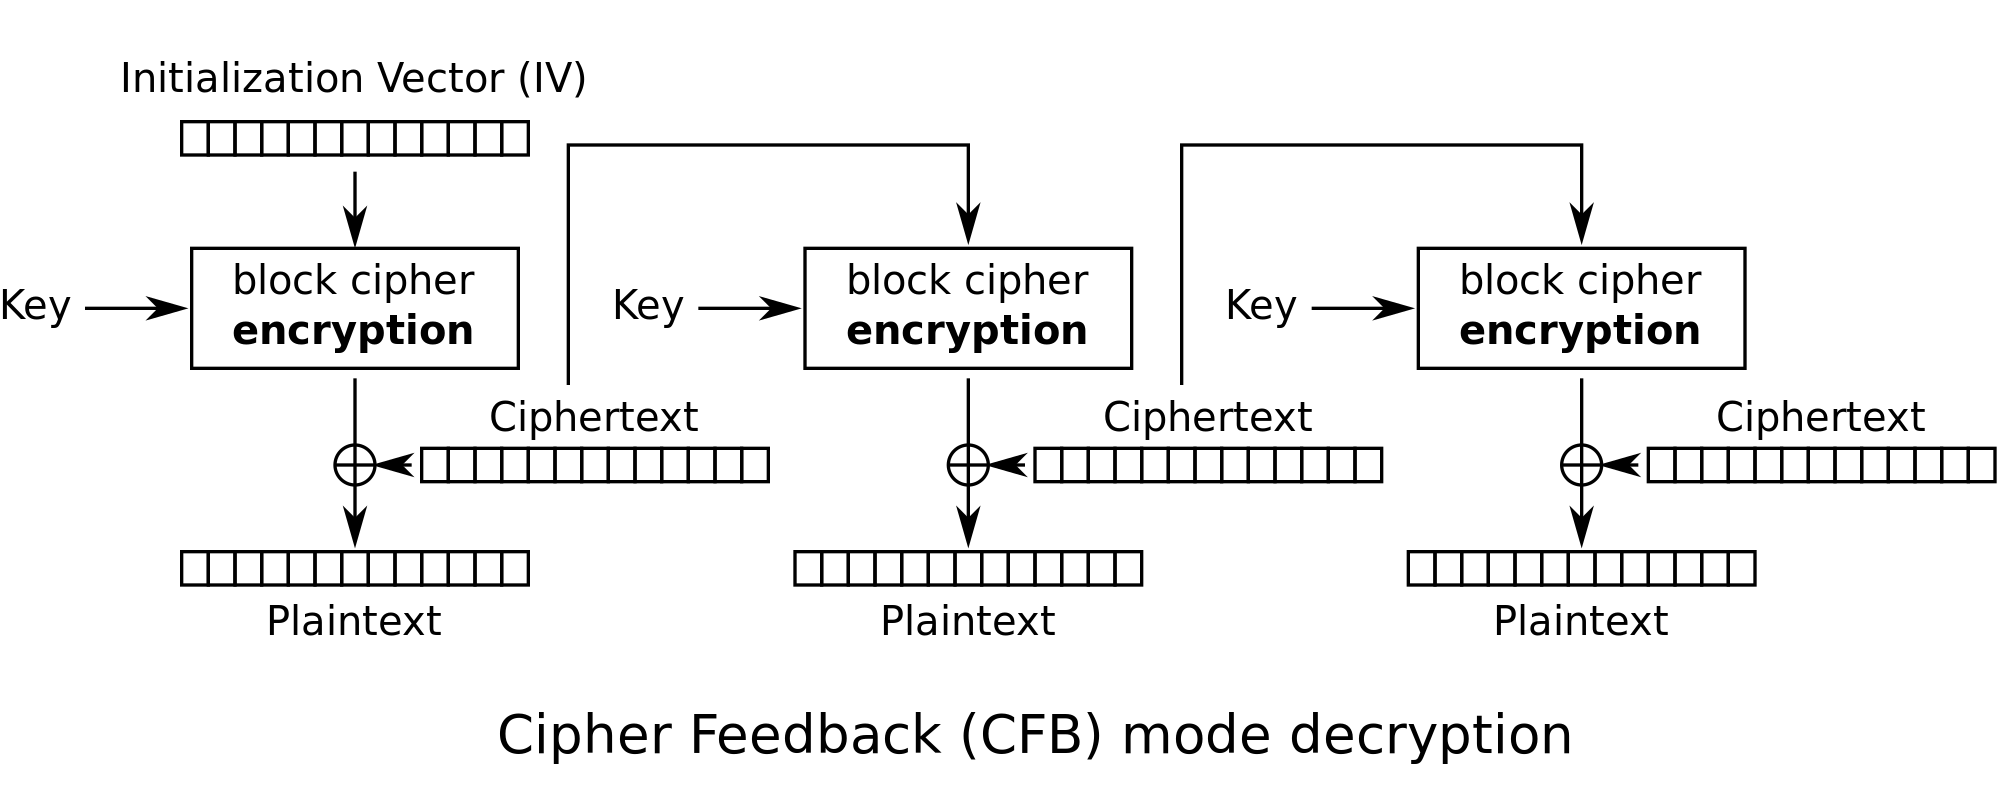
\includegraphics[scale=0.2]{img/CFB.png}
\newline 
The Cipher Feedback (CFB) mode, a close relative of CBC, makes a block cipher into a self-synchronizing stream cipher. Operation is very similar; in particular, CFB decryption is almost identical to CBC encryption performed in reverse.
By definition of self-synchronising cipher, if part of the ciphertext is lost (e.g. due to transmission errors), then receiver will lose only some part of the original message (garbled content), and should be able to continue correct decryption after processing some amount of input data.\\\\
Remarks:
\begin{itemize} 
\item 8 bits encrypted at a time. Then there is a shift in the IV. The image above is too generic.  
\item Another important problem is the error propagation: if I receive for instance $\bar{c}_1,c_2..,c_n$ then I can not decrypt anything! This problem is solved with OFB because the 8-bits are used in the next IV before being XORed with the PT
\item It is used for video.
\end{itemize}
\subsection{Output Feedback (OFB)}
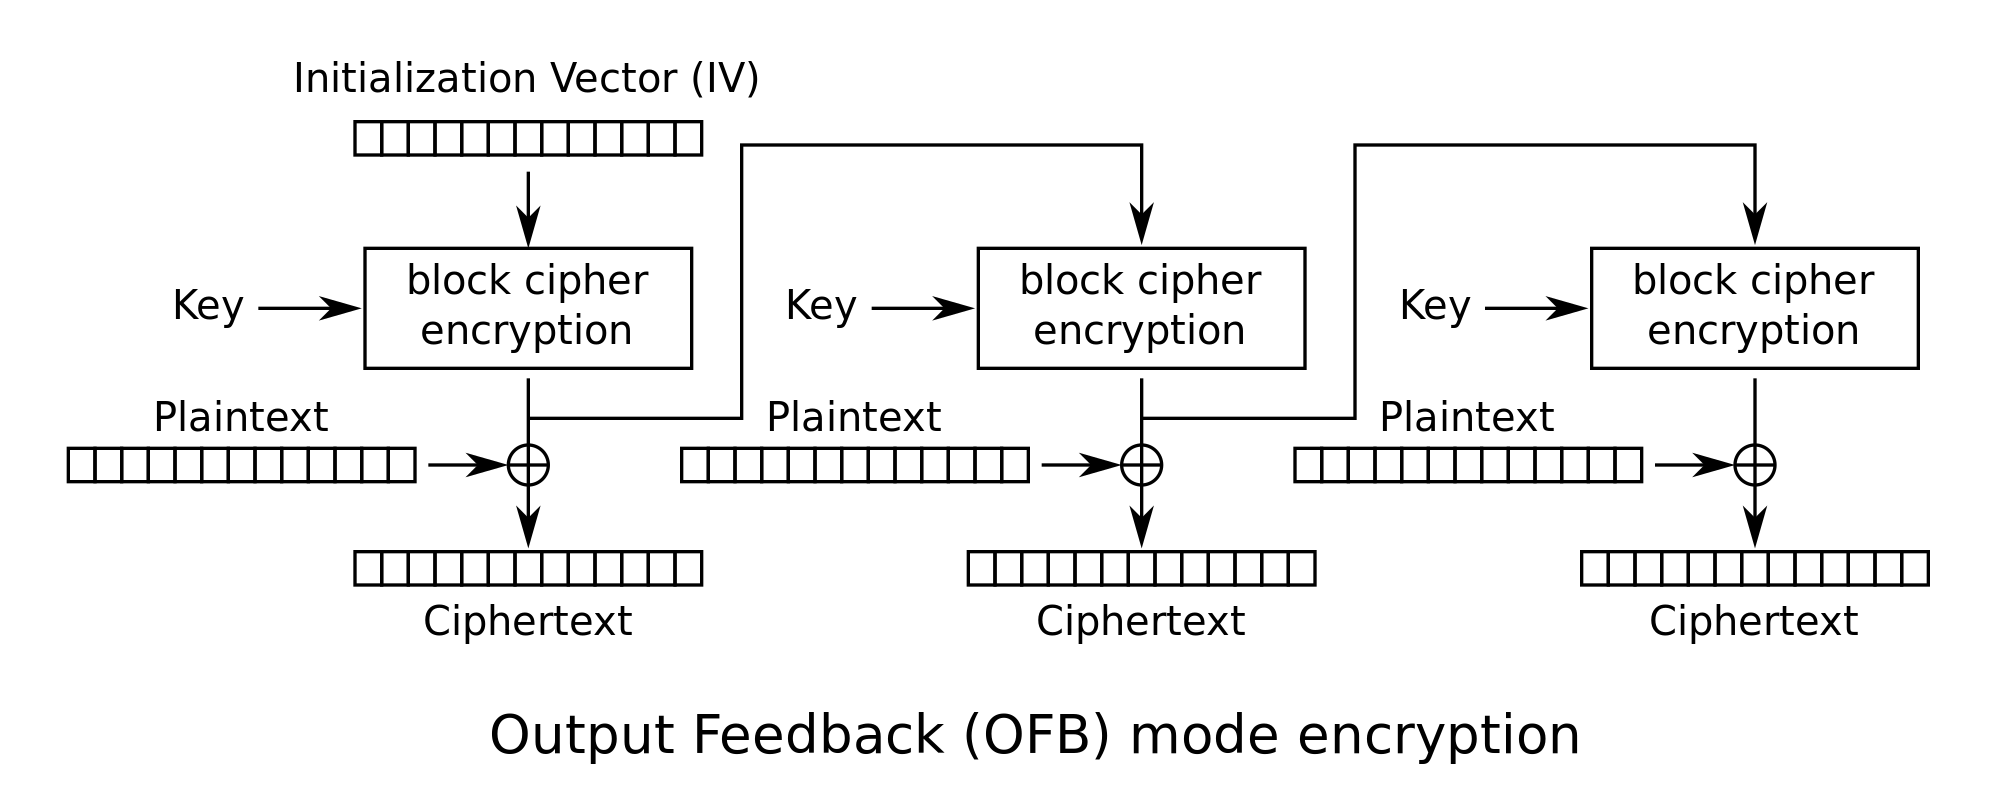
\includegraphics[scale=0.2]{img/OFB.png}
\newline 
The Output Feedback (OFB) mode makes a block cipher into a synchronous stream cipher. It generates keystream blocks, which are then XORed with the plaintext blocks to get the ciphertext. Just as with other stream ciphers, flipping a bit in the ciphertext produces a flipped bit in the plaintext at the same location. This property allows many error correcting codes to function normally even when applied before encryption.
\begin{remark} this modes corrects the error propagation of CFB however  it is still not parallelizable. Here it comes CTR. \end{remark}
\subsection{Counter (CTR)}
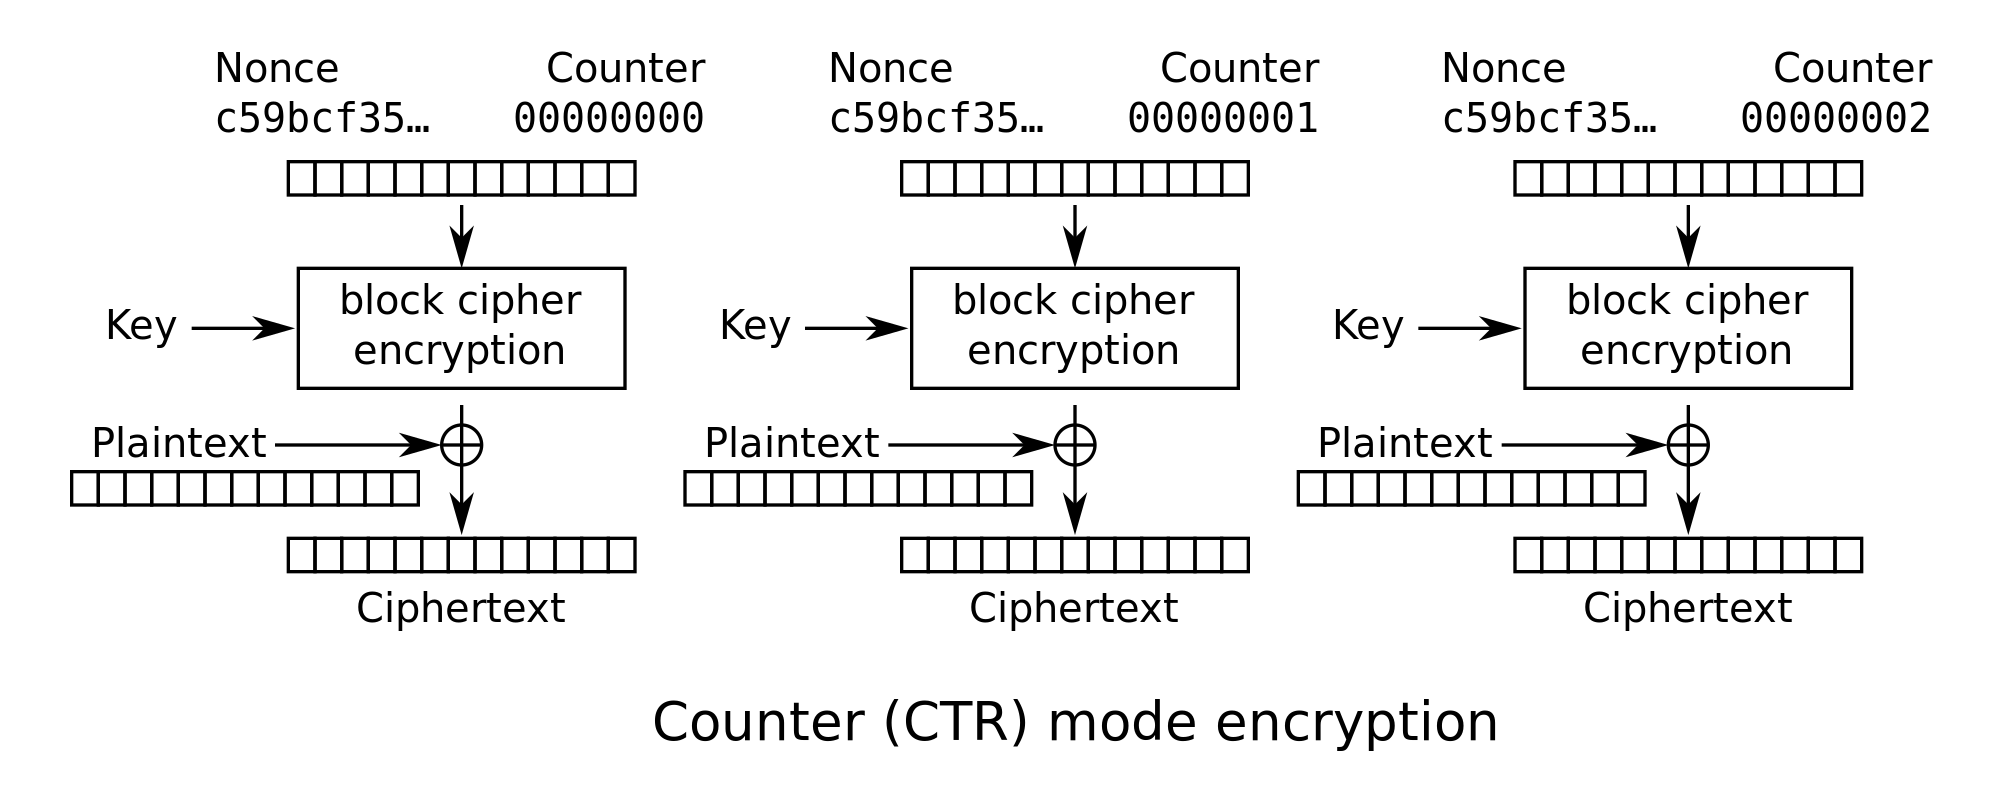
\includegraphics[scale=0.2]{img/CTR.png}
\newline 
Counter mode turns a block cipher into a stream cipher. It generates the next keystream block by encrypting successive values of a "counter". The counter can be any function which produces a sequence which is guaranteed not to repeat for a long time, although an actual increment-by-one counter is the simplest and most popular.
\begin{remark} it is used in ATM, IPSEC. \end{remark}

\begin{remark}
in this mode decryption is performed by swapping around PT and CT hence the block cipher is used only in ecryption mode!
\end{remark}
\subsection{XTS}
The scenario with hard disk is completely different from a TLS connection. With an hard disk there is a huge quantity of information.
In an hard diks a sector is made of blocks.\\
$$Sector_1: [block_1, ... , block_n]$$
$$Sector_2: [block_1, ... , block_n]$$
{\bf Problem 1:} the same info can be saved in different blocks or in different sectors in the same way. It is the same issue of ECB. To overcome this problem the encryption depends on the sector number $i$ and block number $j$.\\\\
Definitions:
\begin{itemize}
\item $Key = Key_1 || Key_2$
\item $P_j$: j-th block of PT. All blocks except possibly the last one have length 128 bits.
\item $C_j$: j-th block of CT. All blocks except possibly the last one have length 128 bits.
\item i: sector number
\item j: block number
\item $\alpha$ primitive element in $GF(2^128)$
\item $\otimes$: modular multiplication of two polynomials  modulo $x^{128}+x^7+x^2+x+1$
\end{itemize}
\begin{center}
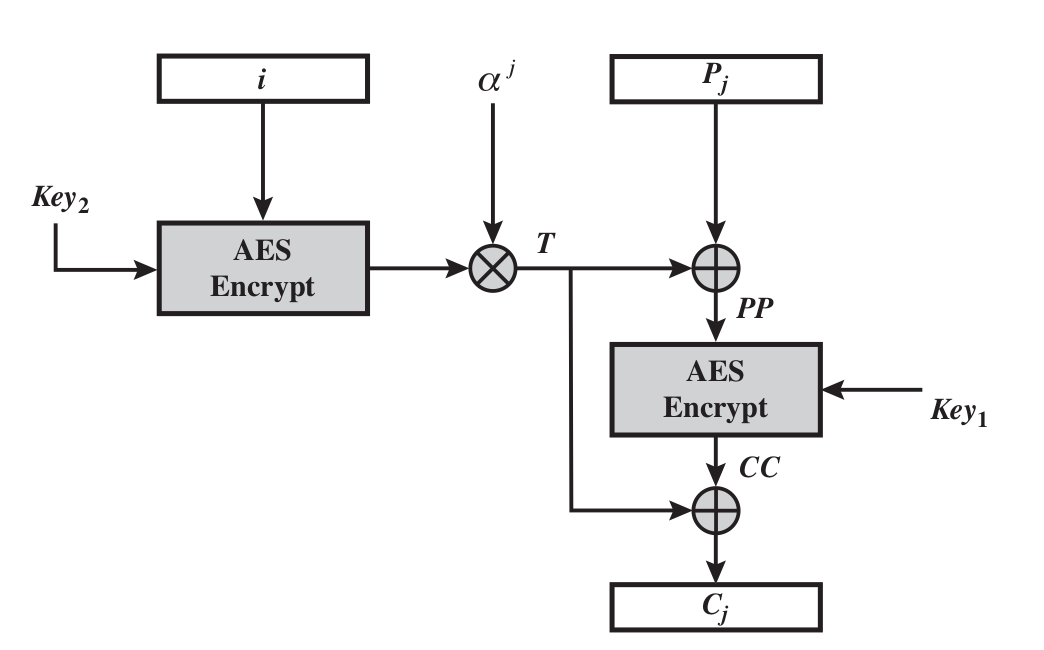
\includegraphics[scale=0.3]{img/XTS-encryption.png}
\end{center}
XTS\_AES block operations:
\begin{itemize}
\item $T = E(K_2,i) \otimes \alpha^j$
\item $PP = P \oplus T$
\item $CC = E(K_1,PP)$
\item $C = CC \oplus T$
\end{itemize}
\newpage
\textbf{Problem 2:} consider encrypting a file of 129 bits with a block size of 128 bits. How is it possible to keep safe even the last bit which is saved in a new block?
\begin{center}
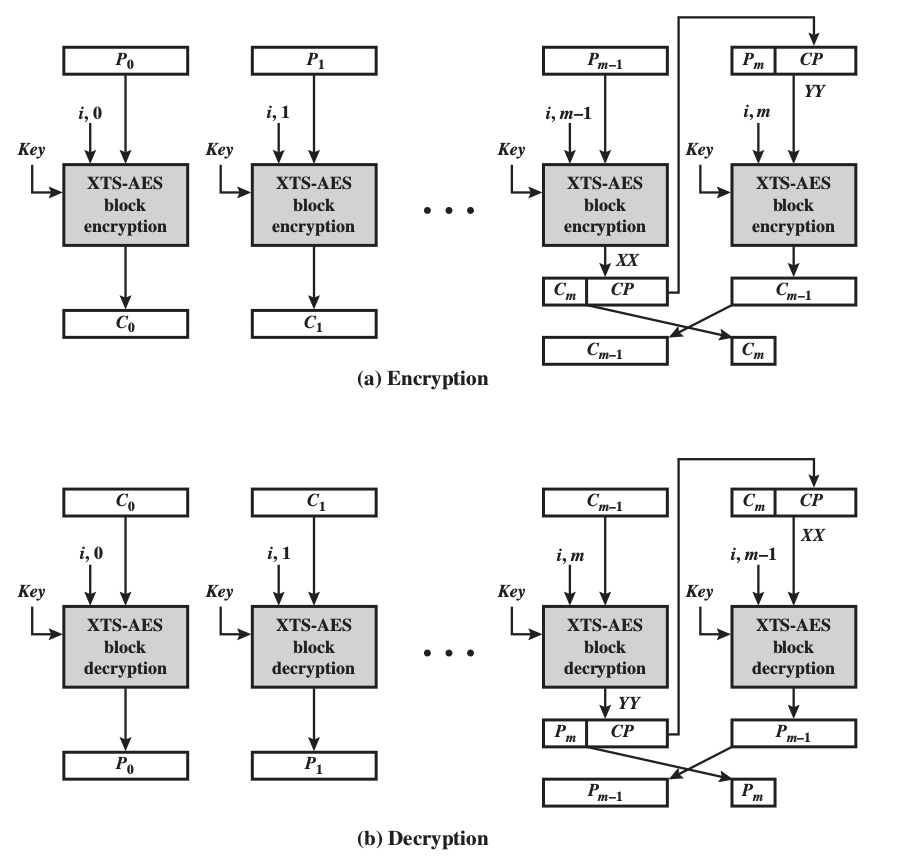
\includegraphics[scale=0.45]{img/XTS-mode.png}
\end{center}
\newpage
\section{Cryptographic hash functions}
\begin{itemize}
\item SHA-2, SHA-3
\item Scrypt
\item Argon
\item BLAKE
\end{itemize}
\subsection{MAC - Message Authentication Code}
A MAC algorithm, sometimes called a keyed (cryptographic) hash function accepts as input a secret key and an arbitrary-length message to be authenticated, and outputs a MAC. The MAC value protects both a message's data integrity as well as its authenticity, by allowing verifiers (who also possess the secret key) to detect any changes to the message content.
\begin{remark}
MACs differ from digital signatures as MAC values are both generated and verified using the same secret key. This implies that the sender and receiver of a message must agree on the same key before initiating communications, as is the case with symmetric encryption. For the same reason, MACs do not provide the property of non-repudiation offered by signatures specifically in the case of a network-wide shared secret key
\end{remark}
\section{Digital Signature}
A digital signature is a mathematical scheme for demonstrating the authenticity of a digital message or documents. Digital signature provides
\begin{itemize}
\item {\bf Authentication:} the recipient has reason to believe that the message was created by a known sender
\item {\bf Non repudiation:} the sender cannot deny having sent the message
\item {\bf Integrity:} the message was not altered
\end{itemize}
Some algorithms:
\begin{itemize}
\item RSA
\item ECDSA
\end{itemize}
\section{Key derivation function}
\section{Certificates}
\subsection{Certificate pinning}
\end{document}